% The \phantomsection command is needed to create a link to a place in the document that is not a
% figure, equation, table, section, subsection, chapter, etc.
%
% When do I need to invoke \phantomsection?
% https://tex.stackexchange.com/questions/44088/when-do-i-need-to-invoke-phantomsection
\phantomsection

% ---
\chapter{Resultados}
\label{cap:resultados}
\phantomsection

Este capítulo apresenta as plataformas de execução das aplicações, aplicações utilizadas, o estudo empírico do número de iterações internas ($t^\prime$), o impacto do tamanho do \tile no desempenho e os resultados da avaliação de desempenho e consumo energético obtidos, comparando-os com a versão \ipc apresentada em~\cite{Podesta:TCC} e com implementações disponíveis no \pskel para plataformas \multicore (\cpu) e \gpu.

\section{Plataformas}
\label{sec:plataformas}

No \mppa, as medições referentes ao consumo de energia foram coletadas através de sensores disponíveis na plataforma, que englobam os \clusters, a memória (\lpddr e memória local de cada \cluster), subsistemas de \io e a \noc. A compilação foi realizada utilizando GCC 5.4 (\mppa e \cpu) e NVCC versão 8.0 (\gpu) com as \textit{flags} de otimização \texttt{-O3} (todas as plataformas), \texttt{-march=native -mtune=native -ftree-vectorize} (\cpu e \gpu) e \texttt{-arch=sm\_35} (\gpu). As implementações para \cpu e \gpu foram executadas nas plataformas abaixo descritas.

\begin{itemize}

  \item \textbf{\xeon}: servidor \textit{desktop} com processador Intel Xeon E5-2640 v4 (Broadwell) de 10 núcleos físicos executando a 2.4 GHz e 64 GB de RAM. As medições de energia nesta plataforma utilizaram a \textit{interface} \rapl da Intel, que considera o consumo de energia de componentes de \hw através de contadores físicos. Esta \textit{inteface} forneceu o consumo de energia da unidade de processamento e da memória.

  \item \textbf{\tesla}: placa gráfica NVIDIA Tesla K40c com 2880 núcleos CUDA de processamento paralelo, executando a 745 MHz e com 12 GB de memória GDDR5. As medições de energia foram obtidas por intermédio da biblioteca de gerenciamento da NVIDIA (\nvml). A \nvml foi usada para obtenção do uso de energia da \gpu e seus circuitos associados (\eg memória interna).

\end{itemize}

\section{Aplicações}
\label{sec:aplicacoes}

As aplicações utilizadas foram \textit{Fur}, \textit{GoL}, \textit{Jacobi} e \textit{Convolution}. Sendo as três primeiras utilizadas na comparação \async \textit{vs.} \ipc e as três últimas na comparação \async \textit{vs.} \gpu \textit{vs.} \cpu.

\begin{itemize}
  \item \textbf{\textit{Fur}}: é um modelo que implementa a maneira como os padrões de pele (listras das zebras, manchas dos leopardos e girafas) nos animais se auto-organiza. Foi primeiramente proposto por Alan Turing. A ideia é que esses padrões são formados individualmente em cada animal, e são influenciados por células de pigmentação presentes no pelo que irão influenciar outras células de pigmentação na sua vizinhança. Dessa maneira, cada animal possui um padrão diferente, mas como as células que irão definir esses padrões são herdadas dos pais, o desenvolvimento desses padrões faz com que os filhotes produzam padrões semelhantes com o de seus pais~\cite{NetLogoFur}. Assim, esta aplicação modelará a pele do animal em uma matriz bidimensional de células de pigmento que podem estar em um dos dois estados: colorida ou não-colorida. Esses estados serão influenciados pela presença de ativadores e inibidores produzidos pelas células da vizinhaça, no qual um nível mais alto de ativadores coloca a célula no estado colorida, um nível mais alto de inibidores leva a célula ao estado de não-colorida e o nível igual de inibidores e ativadores não muda o estado da célula.

  \item \textbf{\textit{GoL (Game of Life})}: é um autômato celular que implementa o Jogo da Vida de Conway~\cite{gardner70}. O autômato é representado por uma matriz na qual cada célula representa um indivíduo no estado vivo ou morto. Com o passar das gerações (iterações), cada célula terá seu estado recalculado de acordo com sua vizinhança. Existem três possíveis ocorrências com o estado de cada célula. Primeiro, o estado permanece inalterado, quando a célula estiver morta e possuir um número de vizinhos vivos diferente de 3, ou a célula está viva e possuir 2 ou 3 vizinhos vivos. Segundo, o estado se altera de morto para vivo, quando uma célula morta possui exatamente 3 vizinhos vivos (``reprodução''). Terceiro, uma célula viva morre, quando a célula viva possui menos de 2 vizinhos vivos (``solidão'') ou mais de 3 vizinhos vivos (``escassez de recursos para sobrevivência'')~\cite{CPE:CPE3479}. 
  
  \item \textbf{\textit{Jacobi}}: Método iterativo para resolver sistemas de equações lineares~\cite{demmel97}.
  O método converge garantidamente se a matriz de entrada é restrita ou irredutivelmente dominante diagonalmente, i.e., $|u_{i,i}| > \sum_{j\neq i}{|u_{i,j}|}$, para todo $i$.
  A Equação~\ref{eq:JacobiPoisson} define a computação em cada passo do método iterativo de Jacobi para resolver a equação discreta elíptica de Poisson~\cite{demmel97}. A solução aproximada é computada discretizando o problema na matriz em pontos espaçados de forma equivalente por $n\times n$.\\
   \begin{equation}
   u'_{i,j} = \frac{u_{i\pm1,j} + u_{i,j\pm1} + h^2f_{i,j}}{4}
   \label{eq:JacobiPoisson}
   \end{equation}
   A cada passo, o novo valor de $u_{i,j}$ é obtido fazendo a média $h^2f_{i,j}$ dos seus vizinhos, onde $h = \frac{1}{n+1}$ e $f_{i,j} = f(ih,jh)$,
   para uma dada função $f$~\cite{Podesta:TCC}.

  \item \textbf{\textit{Convolution}}: a convolução é uma técnica utilizada em diversas áreas de estudos. No processamento digital, é possível utilizá-la para realizar filtros de sinais, e assim atenuar ou realçar um áudio, uma imagem ou até mesmo um vídeo. O processo de convolução em uma imagem digital, recebe uma imagem $\mathit{I}$ de largura $\mathit{W}$ e altura $\mathit{H}$ e a transforma em uma imagem $\mathit{O}$ de mesma dimensão. Uma matriz $\mathit{M}$ de coeficientes é utilizada em conjunto com a imagem a ser processada para cálcular a imagem resultante~\cite{CPE:CPE3479}.
\end{itemize}

\section{Estudo empírico: iterações internas (\texorpdfstring{$t^\prime$}{t'})}
\label{sec:tam_tile_alargado}

Devido ao uso da técnica de \textit{tiling} trapezoidal, é possível definir com precisão o tamanho da \textit{ghost zone} mediante o parâmetro $t^\prime$. Essa é uma característica importante, que permite explorar a baixa quantidade de memória presente nos \clusters e fazer melhor uso da \noc, pois a \textit{ghost zone} impacta diretamente no tamanho e no consumo de memória do \tile alargado. Assim, um estudo empírico com as aplicações supracitadas fora realizado para definir um valor ótimo para esse parâmetro. A Figura~\ref{fig:tprime} expõe o ganho de desempenho quando variado o valor de $t^\prime$ no intervalo de $2$ a $16$ (o ganho de desempenho é em relação a $t^\prime=1$). Como já mencionado, existe um \textit{tradeoff} entre o custo da computação redundante e a redução de comunicação e sincronização na \noc. O estudo empírico mostra que o melhor \textit{tradeoff} é alcançado com $t^\prime=10$. Devido a isso, os resultados obtidos nas seções seguintes utilizam $t^\prime=10$.

\begin{figure}
  \centering
	\caption{Estudo empírico para encontrar o melhor valor para $t^\prime$. Melhor troca é alcançada com $t^\prime=10$.}
	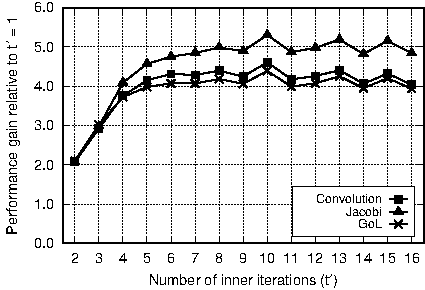
\includegraphics[width=0.7\textwidth]{figs/MPPAPlotIterationsAPI100It16InnerIt.pdf}
	\label{fig:tprime}
\end{figure}

\section{Tamanho do \tile \textit{vs.} desempenho}
\label{sec:tam_tile_desempenho}

Nesta seção é analisado o impacto do tamanho do \tile no desempenho das aplicações do \pskel no \mppa com a versão \async. Foram considerados quatro tamanhos de dados de entrada (\ina, \inb, \inc, \ind) e quatro tamanhos de \tiles (\tilea, \tileb, \tilec, \tiled). Estes tamanhos máximos foram cuidadosamente selecionados para não extrapolar a quantidade de memória disponível para uso no \mppa (2GB na \lpddr e 2MB em cada \cluster). O número de iterações utilizado foi $t = 100$. Os resultados obtidos representam a media de 20 execuções com o desvio padrão médio menor que $1\%$. 

A Figura~\ref{fig:tiles} mostra o desempenho das aplicações estêncil quando variado o tamanho do dado de entrada e o tamanho do \tile. Ao dobrar o tamanho da entrada observa-se um aumento médio de 2x a 3,3x no tempo de execução. Este comportamento é esperado, pois com o aumento da quantidade de dados mais computações, comunicações e sincronizações são necessárias.

Outrossim, é observado que ao aumentar o tamanho do \tile o desempenho das aplicações é muito beneficiado, independente do tamanho do dado de entrada. Isto está vinculado à duas circunstâncias. Primeiro, a redução do número de operações de escrita/leitura e sincronizações entre o subsistema de \io e os \clusters por meio da \noc. Isso permite que maiores transferências de dados sejam realizadas por operação de escrita/leitura, otimizando a taxa de transferência da \noc. Segundo, maiores \tiles significam maior paralelismo dentro dos \clusters de computação (\ie \textit{threads} OpenMP possuirão mais trabalho para computar), reduzindo o \textit{overhead} proveniente das regiões paralelas do OpenMP. Ao variar o tamanho do \tile de \tilea para \tileb, foram observados ganhos de até 3x em todas as aplicações. O ganho de desempenho aumentou em pelo menos 6,9x e 10,3x quando o tamanho do \tile foi variado de \tilea para \tilec e de \tilea para \tiled, respectivamente.

\begin{figure}
  \centering
  \caption{\textit{Tiles} vs. tempo de execução}
  \begin{subfigure}{0.338\textwidth}
    \centering
    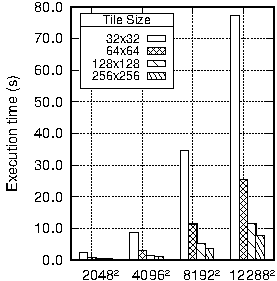
\includegraphics[width=1\textwidth]{figs/MPPAPlotAPIconvolutionTimeTiles.pdf}
    \caption{\convolution}
    \label{fig:tilesConvolution}
  \end{subfigure}
  \begin{subfigure}{0.3\textwidth}
    \centering
    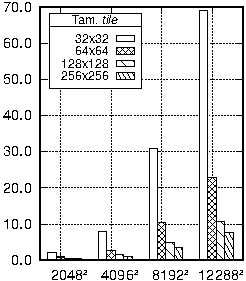
\includegraphics[width=1\textwidth]{figs/MPPAPlotAPIgolTimeTiles.pdf}
    \caption{\gol}
    \label{fig:tilesGol}
  \end{subfigure}
  \begin{subfigure}{0.3\textwidth}
    \centering
    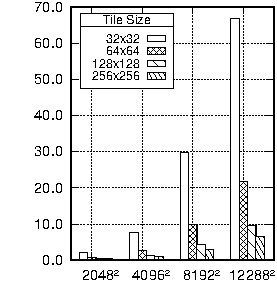
\includegraphics[width=1\textwidth]{figs/MPPAPlotAPIjacobiTimeTiles.pdf}
    \caption{\jacobi}
    \label{fig:tilesJacobi}
  \end{subfigure}
  \label{fig:tiles}
\end{figure}


\section{Análise de escalabilidade}
\label{sec:analise_escalabilidade}

Nesta seção será analisada a escalabilidade do \pskelmppa na versão \async. A Figura~\ref{fig:escalabilidade} mostra o tempo de execução de cada aplicação no \mppa, variando o número de \clusters de computação utilizados de $1$ a $16$. Neste experimento, foi utilizado o número de iterações $t=100$, o tamanho do dado de entrada e do \tile de \ind e \tiled, respectivamente. Como pode ser visto, as três aplicações estêncil possuem comportamento semelhante e tem o tempo de execução reduzido a medida que o número de \clusters utilizados aumenta. Foi observada uma aceleração de 15,3x quando comparado o uso de 16 \clusters em relação a apenas um \cluster. Isso mostra que a versão \pskelmppa \async consegue explorar o uso de todas as fontes de computação e o uso da \noc do \mppa.

\begin{figure}
	\centering
	\caption{Escalabilidade.}
	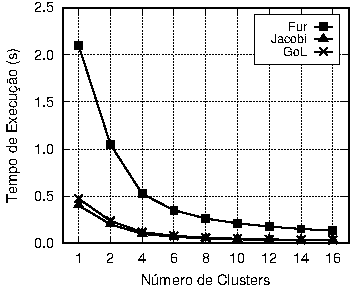
\includegraphics[width=.6\textwidth]{figs/MPPAPlotScalabilityAPI.pdf}
	\label{fig:escalabilidade}
\end{figure}

\section{\mppa \async \textit{vs.} \mppa \ipc}
\label{sec:async_vs_ipc}

Esta seção apresenta a comparação entre a nova versão do \pskelmppa (\async) com a versão antiga do \pskelmppa (\ipc). 
A \autoref{fig:async_vs_ipc} apresenta a comparação de tempo de execução e consumo de energia entre ambas versões.
Nesse experimento, foi utilizada uma matriz de dados de tamanho \ind, \tiles de tamanho \tilec e \tiled (apenas para a \async), 16 \clusters e 16 \pes por \cluster.
A versão \ipc recorria à alocação de dados temporários para auxiliar no envio/recebimento de dados dos \clusters de computação, consumindo parcela significativa da já escassa memória local e limitando o tamanho máximo dos \tiles.
Esta prática foi descontiuada na versão \async com o uso da nova \api, viabilizando o aumento do tamanho máximo dos \tiles para \tiled.
O número de iterações utilizado foi $t = 30$. Os resultados obtidos representam a média de 5 execuções com o desvio padrão médio menor que $1\%$, o número de iterações e execuções visa manter paridade com os resultados gerados na versão \ipc~\cite{Podesta:TCC}. 

\begin{figure}[t]
  \centering
  \caption{\async \textit{vs.} \ipc}
  \begin{subfigure}{0.494\textwidth}
    \centering
    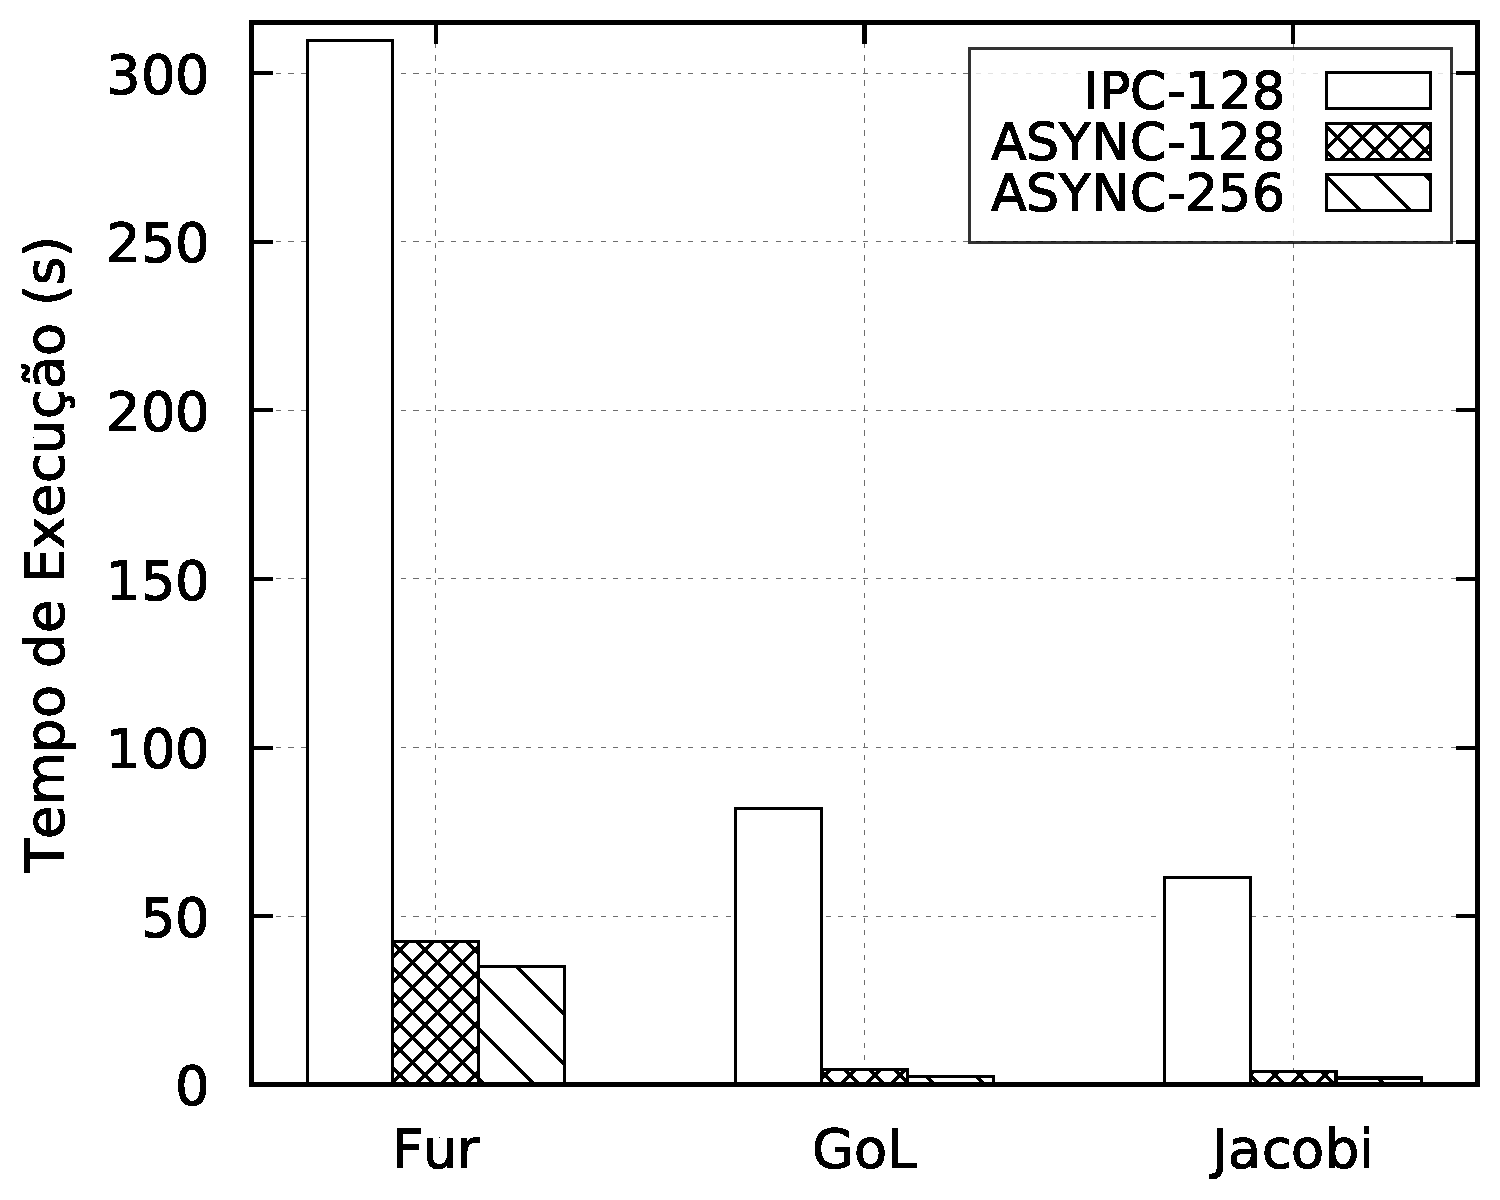
\includegraphics[width=1\textwidth]{figs/ipc_vs_async_exec_time.pdf}
    \label{fig:compara-tempo}
  \end{subfigure}
  \begin{subfigure}{0.494\textwidth}
    \centering
    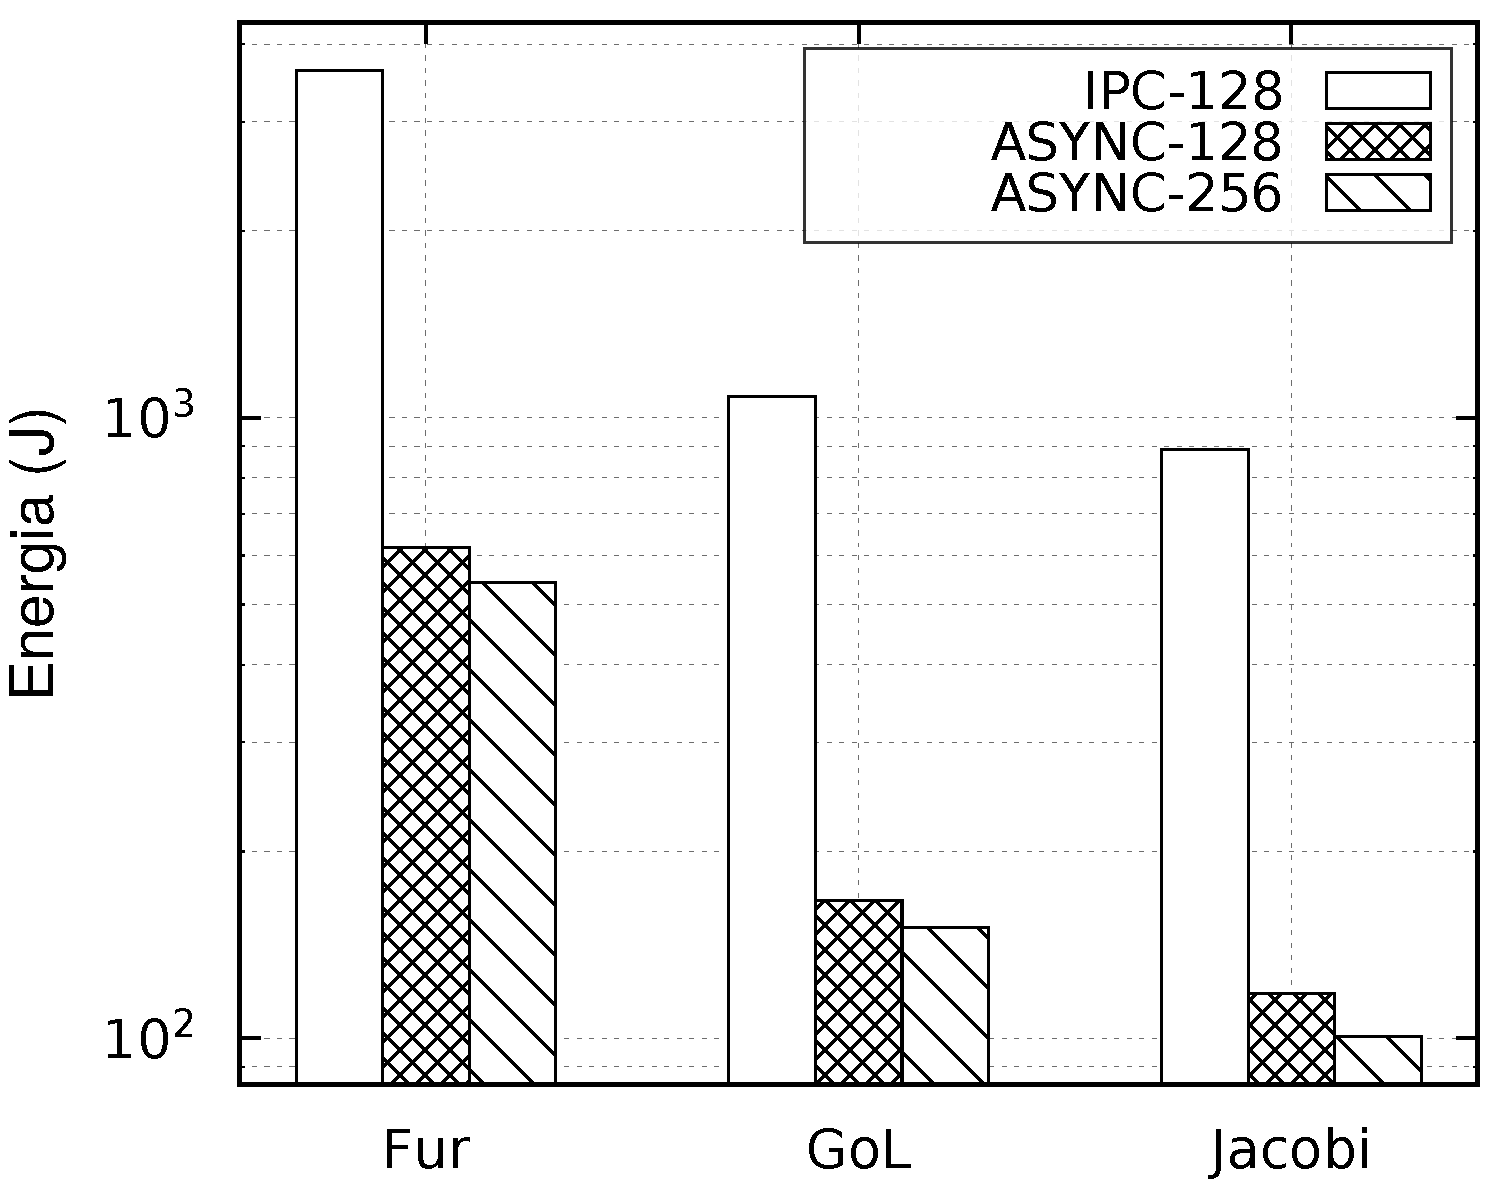
\includegraphics[width=1\textwidth]{figs/ipc_vs_async_energy.pdf}
    \label{fig:compara-energia}
  \end{subfigure}
  \label{fig:async_vs_ipc}
\end{figure}

O tempo de execução da versão \async é de 8.86x, 33.48x e 30.29x mais rápido que o tempo de execução da versão   \ipc, para as aplicações \fur, \gol e \jacobi, respectivamente. Essa diferença está correlacionada ao fato da versão \async fazer melhor uso da \noc na distribuição dos dados para os \cluster de computação e realizar menos sincronizações entre mestre e trabalhador. Além disso, otimizações na computação como a verificação de elementos presentes nas bordas de computação também contribuem para este resultado.

O consumo de energia segue um comportamento similar, uma vez que, menos tempo executando acarreta em menos tempo consumindo energia. Assim, é apresentada uma eficiência no consumo de energia superior em até 8.84x a favor da versão \async.

\begin{figure}[t]
  \centering
  \caption{\mppa \async \textit{vs.} \cpu \textit{vs.} \gpu.}
  \begin{subfigure}{0.494\textwidth}
    \centering
    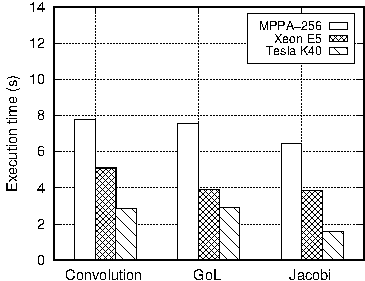
\includegraphics[width=1\textwidth]{figs/ComparisonTimeTiles10.pdf}
    \label{fig:compara-tempo-async-cpu-gpu}
  \end{subfigure}
  \begin{subfigure}{0.494\textwidth}
    \centering
    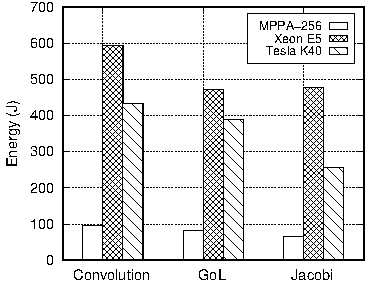
\includegraphics[width=1\textwidth]{figs/ComparisonEnergyTiles10.pdf}
    \label{fig:compara-energia-async-cpu-gpu}
  \end{subfigure}
  \label{fig:async_vs_cpu_gpu}
\end{figure}

\section{\mppa \async \textit{vs.} \cpu \textit{vs.} \gpu}
\label{sec:async_vs_cpu_gpu}

Por fim, é comparado o tempo de execução e consumo de energia obtido com o \pskelmppa \async em relação as implementações do \pskel para \cpu e \gpu. Foi utilizado dados de entrada de tamanho \ind e \tiles de tamanho \tiled, a escolha do tamanho dos \tiles foi baseada no melhor desempenho obtido na Figura~\ref{fig:tiles}. Com o objetivo de realizar uma comparação justa, foram utilizadas as melhores otimizações disponíveis para o \xeon e \tesla, presentes nos \textit{back-ends} de \multicore e \gpu do \pskel. O número de iterações utilizado foi $t = 100$, utilizando os 16 \clusters e 16 \pes por \cluster. Os resultados obtidos representam a media de 20 execuções com o desvio padrão médio menor que $1\%$. A Figura~\ref{fig:async_vs_cpu_gpu} apresenta os resultados obtidos.

De modo geral, o \pskelmppa \async é competitivo quanto ao tempo de execução porém fica atrás das implementações para \cpu e \gpu. O tempo de execução das aplicações \convolution, \gol e \jacobi no \mppa foi de 1.52x, 1.93x e 1.67x maior em relação a \cpu, de  e 2.72x, 2.61x e 4.04x maior em relação a \gpu, respectivamente.

No consumo de energia o \pskelmppa \async obteve os melhores resultados em todas as aplicações. O principal motivo é que o próprio \mppa oferece uma arquitetura altamente paralelizável e com baixo consumo de energia. Ainda assim, a técnica de \textit{tiling} trapezoidal utilizada~\cite{Podesta:TCC}, a implementação com a nova \api de comunicação \async e as otimizações realizadas foram de extrema importância para obtenção desse desempenho no consumo energético. O consumo de energia no \mppa foi de até 7.34x e 4.71x menor do que o da \cpu e \gpu, respectivamente.
